\documentclass[letterpaper,12pt]{article}

% csm-thesis automatically includes the following packages:
%% float
%% setspace
%% geometry
%% graphics
%% textcase
%% subfig

% Note: Two package options exist for your convenience: ``insane'' and ``nolabel''.  To use these options together separate them by a comma, ie. \usepackage[insane,nolabel]{csm-thesis}
% * \usepackage[insane]{csm-thesis}
% Turn off all document sanity checks.  This option can be used to render a ``sub-document'' that is part of the root thesis document.  It is important to note that you should NEVER disable this check on your root thesis document, as important format errors and warnings will be disabled.
% * \usepackage[nolabel]{csm-thesis}
% Disables automatic reference ``labeling'' of figures and tables.  By default the thesis template prepends any reference to a figure or table with ``Figure~'' or ``Table~''.  This option is meant for disabling the labeling behavior when a document already has the appropriate labeling.  It is important to note that if your document DOES NOT have the appropriate labeling (the reference label must EXACTLY MATCH the caption label) then it will not pass the format review.
\usepackage{csm-thesis}

% For inserting large multi-page tables:
\usepackage{array}
\usepackage{longtable}

% For inserting sideways tables and figures
\usepackage{rotating}
\usepackage[numbers]{natbib}
\graphicspath{{./images/}}
\usepackage{hyperref}

% For inserting programming code:
\usepackage{listings}

% For inserting landscape-mode objects:
\usepackage{pdflscape} % use ``lscape'' if you are not creating a PDF output

% For matrices:
\usepackage{amsmath}

\title{Come up with a thesis title}

\degreetitle{Doctor of Philosophy}
\discipline{Computer Science}
\department{Electrical Engineering and Computer Science}

\author{James Howard}
\advisor{Dr. William Hoff}
\dpthead{Dr. Big Boss}{Professor and Head}

\begin{document}

% Parts of a Thesis
\frontmatter

\maketitle
\newpage

%%%% Parts of a Thesis - Front Matter - Copyright Page (optional)
%% If the copyright for your document spans multiple years, or does not match the current year, then replace ''\the\year`` below with the appropriate text.
\makecopyright{\the\year}
\newpage

%%% Parts of a Thesis - Front Matter - Signature Page (required)

\makesubmittal
\newpage

%%% Parts of a Thesis - Front Matter - Abstract (required)
\begin{abstract}
Forecasting the occupancy of buildings can lead to significant improvement of smart heating and cooling systems. Using a sensor network of simple passive infrared motion sensors densely placed throughout a building, we perform data mining to forecast occupancy a short time ($i.e.$, up to 60 minutes) into the future.  Our approach is to train a set of standard forecasting models to our time series data.  Each model then forecasts occupancy a various horizons into the future.  We combine these forecasts using a modified Bayesian combined forecasting approach.  The method is demonstrated on two large building occupancy datasets, and shows promising results for forecasting horizons of up to 60 minutes.  Because the two datasets have such different occupancy profiles, we compare our algorithms on each dataset to evaluate the performance of the forecasting algorithm for the different conditions.
\end{abstract}

\newpage

%%% Parts of a Thesis - Front Matter - Table of Contents (required)

\tableofcontents
\newpage

%%% Parts of a Thesis - Front Matter - List of Figures (if applicable)
%%% Parts of a Thesis - Front Matter - List of Tables (if applicable)

\listoffiguresandtables
\newpage

%\listofsymbols
%Place symbols here

\newpage

%%% Parts of a Thesis - Front Matter - List of Abbreviations (if applicable)
\listofabbreviations*
\newpage

\addabbreviation{Seasonal Auto Regressive Moving Average Model}{SARIMA}

%%% Parts of a Thesis - Front Matter - Acknowledgments (optional)
\begin{acknowledgments}
That you everyone
\end{acknowledgments}
\newpage

%%% Parts of a Thesis - Front Matter - Dedication (optional)

\begin{dedication}
For those that shall follow after.
\end{dedication}
\newpage

% Parts of a Thesis - Body

\bodymatter

%%% Parts of a Thesis - Body - All Chapters and Sections (required)
%Introduction
\chapter{Introduction}
According to the U.S. Department of Energy \cite{DOE2010} energy for heating and cooling accounts for approximately 35 - 45\% of the total expenditure within a building.  With such a large investment of energy being used to regulate the temperature of a building, any possible areas of improvement in this area are heavily sought after.  One idea for saving energy is to only regulate the temperature in rooms that are actually in use.  While the problem of determining what rooms are in use can be solved easily by a motion sensor, this problem becomes more difficult when the lead time to heat or cool a room is considered.  If accurate forecast models could be made for the occupancy of any section of the building, then a control scheme may be created that could save on total energy cost.

As another example where the forecasting of occupancy may be used to produce significant improvements, consider the roadways of the United States.  Optimal timing of traffic lights on major roadways across the United States could account for approximately a 22\% reduction in emissions along with a 10\% reduction in fuel consumption \cite{DOT2007}.  As of 2005 the total estimated fuel savings would amount to approximately 17 billions gallons of motor fuels annually.  If accurate estimates of future traffic patterns at each traffic light were available then dynamically changing the light timings to account for such traffic would improve overall traffic flow.

In both of the above scenarios motion through the environment can be captured through a network of many sensors.  For vehicular traffic systems, networks already exist using inductive loops and radar based sensors to count the number of cars in a given unit of time.  In the case of buildings, such networks are not as common.  To acquire such counts one could install a network using many infrared motion sensors and cameras to count human motion through the building.  

%Problem Statement
\subsection{Objective and Approach}
The objective of this work is to forecast the number of moving agents in a region of space $\delta$ seconds in the future.  This could be represented by a hypothesis function $h(x, \delta)$.  We will use mean absolute scale error (MASE) \cite{Hyndman2006} and mean absolute percentage error (MAPE) as  cost functions to compare with other previously implemented techniques.  Due to the level of noise present in traffic scenarios, the forecasted value of a sensor reading is aggregated for a time appropriate for the setting.  For vehicular traffic, most work deals with reading every 15 minutes to one hour.  For building traffic, this aggregation is 3 to 5 minutes.  

To assist in constructing models we make the assumption that data is generated from activities produced by human controlled entities moving through the environment.  Also we assume that the activities are repetitive and on some schedule.  The result of these assumptions is that from such scheduled movement we get sensors which have a spatial correlation and that for example, from week to week on the same day display similar trends.   Much of the research on traffic forecasting makes a similar assumption.  

We also assume that sufficient deviations from our forecasting function are often not the result of noise, but are due to an activity that does not commonly occur on that day.  Because such activities can overlap or occur at different times with varying amount of background noise present, it is a difficult task for one parametric model to accurately encapsulate all possible combinations of activities.  In an environment with many activities that could occur at multiple different times such combinations may be prevalent.  Past work doesn't address the problem of overlapping activities.  
%
%
%\begin{wrapfigure}{r}{5cm}
%\begin{center}
%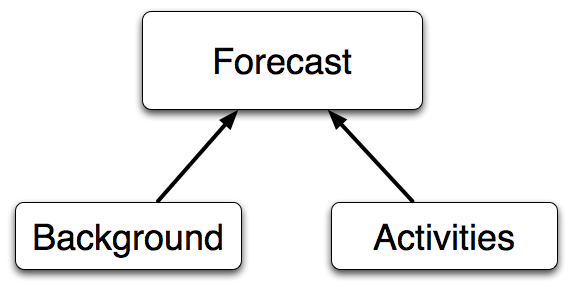
\includegraphics[width=0.30\textwidth]{flow_chart.png}
%\end{center}
%\caption{Forecasting is based on activities and a background model}
%\label{fig:flow_chart}
%\end{wrapfigure}
%
%Our approach is to split the problem of forecasting into two parts: development of a background model and the development of a set of activity models.  Our background model is represented by a seasonal autoregressive integrated moving average (ARIMA) model.  To model activities, we propose comparing different models from activity recognition literature along with a new model which we propose here.  Forecasting is then performed using an ensemble predictor taking outputs from all trained activity models and the background seasonal ARIMA model.
%
%
%%\section{Previous Work}
%%Work in the past has attempted to solve this problem with parametric regression approaches such as fitting an auto regression moving average model (ARMA).  These models use a local history of forecasted values and actual readings to forecast future values.  The primary problem with these approaches is that due to being parametric with the background mean incorporated into the model, they tend to have problems with unusual patterns especially in the presence of changing means.
%
%%There has also been a limited amount of work into using multiple models to predict future observations.  While such work has shown promise, there has also been a lack of research into discovery of the optimal timeframe and spatial influence of other sensors when considering such models.  Other predictive approaches tend to use the entire network.  We instead search for the best spatial features and temporal scales to perform prediction.
%
%
%%Example Activity
%\section{Example Activity}
%
%\begin{figure}[ht]
%\begin{center}
%\subfloat[][Away game Sundays] {
%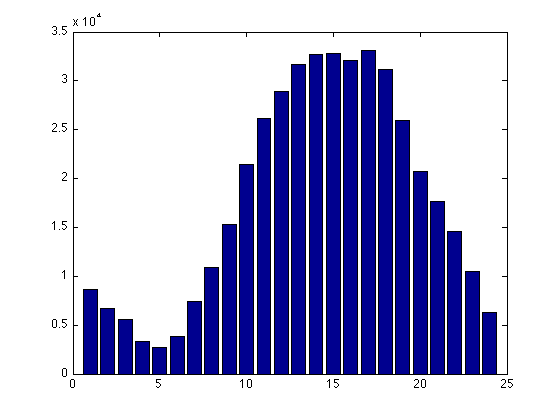
\includegraphics[width=0.45\textwidth]{broncos_off4.png}
%\label{fig:broncos_off}
%}
%\subfloat[][Broncos game Sundays] {
%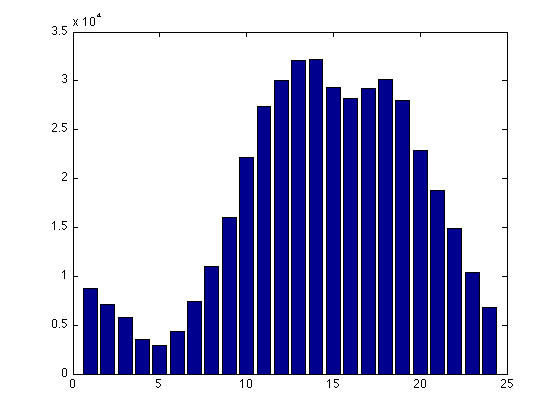
\includegraphics[width=0.45\textwidth]{broncos4.png}
%\label{fig:broncos_on}
%}
%\end{center}
%\caption{Total number of cars passing major highway sensors on Sundays in September and October 2010}
%\label{fig:broncos}
%\end{figure}
%
%To illustrate an example of the need for our approach we provide the following example.  Figure~\ref{fig:broncos} shows the total counts of Denver traffic for each hour of the day averaged for the first four Sunday Broncos home games and for the first four Sunday away games in 2010.  Comparing figure~\ref{fig:broncos_off} with figure~\ref{fig:broncos_on} it is evident that a noticeable change in traffic patterns occur from approximately noon until approximately 6:00 pm.  This traffic change corresponds with a 2:05pm kickoff time for the game. 
%
%Traditional parametric models have difficulty accounting for these different traffic patterns and the problem becomes more difficult when when it is considered that the Broncos may play a Sunday night game or a Monday night game.  To compound the problem further there may be multiple activities occurring at the same time such as a Rockies game and a Broncos game.  It is probable that the number of occurrences of such overlapping activities are few and that no training instances exist for traditional models to handle.  
%
%Our approach will model each discrete activity separately and independent of the background model.  In this case a model for Broncos games and a model for Rockies games would be trained.  Once trained, accurate prediction should be possible despite the time of the games or the presence of other activities.
%
%\section{Contributions}  
%The contributions to the field of unsupervised traffic forecasting from this work are:
%\begin{itemize}
%\item{Use of activity models for improved forecasting accuracy of seasonal ARIMA models.}
%%\item{A combined Bayesian prediction model which uses the results of a background model and activity models to predict future readings.}
%\item{A new representation of activities using a mixture of time series multivariate Gaussians.}
%\item{A new measure for determining activity model forecasting accuracy.}
%\end{itemize}
%
%\section{Structure of the Proposal}
%The remainder of this proposal is outlined as follows.  Section two reviews current work related to traffic prediction and activity modeling.  Section three gives a summary of each dataset used in this work.  Section four details specific pieces of the overall approach.  All of the approach is not solved and where possible this section details potential ways to proceed with each unsolved part of the approach.  Finally section five is a time line of when the remaining work is expected to be completed.
%


\chapter{Datasets}
This chapter contains dataset information

\subsection{Notation}
As already stated, we define a time series dataset used within as  $\{x_{t}^{(m)}\}$.  Each $x_{t}^{m}$ is an aggregate of the readings from sensor $m$ reading at time block $t$. 

Forecasts for a given model $k$ from the set of all models $K$ are represented by 
\begin{equation}
\bar{T}_{t + 1}^{k, m} = f(T_{t}, ..., T_{1}; \theta_{k}).
\end{equation}
\noindent
Thus the forecast of $T_{t + 1}$ is a function of all past data and some trained parameterization $\theta_{k}$ for that model. 

In this work we need to forecast more than one time step into the future.  Future forecasts are performed through iterative one step ahead forecasts.  Also for this work we forecast a model for each individual sensor and for convenience drop the $m$ from our forecasting notation.  An example of a forecast two time steps ahead of current time $t$ is given by 
\begin{equation}
\bar{T}_{t + 2}^{k} = f(\bar{T}_{t + 1}, T_{t}, ..., T_{1}; \theta_{k}).
\end{equation}
\noindent
Such a forecast is simply the forecast for one time step into the future but now with the forecasted value of $\bar{T}_{t + 1}$ used as the most recent datapoint to forecast $\bar{T}_{t + 2}$.  Forecasting in this nature allows for forecasts any number of time steps into the future. 

\subsection{Forecast measurements}
Discuss MAPE, MASE, RMSE, and our approach here

TODO: Perhaps remove this to another section
This could be represented by a hypothesis function $h(x, \delta)$.  We use mean absolute scale error (MASE) \cite{Hyndman2006} and root mean squared error (RMSE) as cost functions to compare with other previously implemented techniques.

\subsection{MERL Dataset} 

The Mitsubishi Electronic Research Labs dataset is derived from a collection of over 200 passive infrared sensors place densely throughout the 7th and 8th floor of a research office building.  The sensors are placed roughly two meters apart on the ceilings, creating a dense sensing area with little non-sensed space.  Readings are taken at the millisecond level, but due to the sensors' settling times the inter-detection time of motion is approximately 1.5 seconds.

The data was collected from March 2006 through March 2008 and there are roughly 53 million sensor readings.  This building is similar to most office buildings with a number of personal offices along with labs and conference rooms.  Employees have roughly set schedules and holidays are observed as normal. 

The counts of sensor activations have been aggregated every 10 minutes.  Because of the lack of significant motion in the night, we look only at activations that occur between 6:00am and 7:00pm daily.  A plot of the average activations of all Wednesdays for a single sensor along with a range of one standard deviation is given in Figure~\ref{fig:merlday}.  

Peak motion unsurprisingly occurs during the middle of the day corresponding to lunch time.  There is another small peak of motion near the start of the day corresponding to people entering.  Near the end of the day, instead of a peak there is a region corresponding to high variance.  This seems to imply that while people enter at roughly the same time, there is a significant variance on when people leave the building.


\subsection{Colorado School of Mines Dataset}

The Colorado School of Mines dataset is a collection of 50 passive infrared sensors mounted on the ceiling of the second floor of a class and office room building.  The density of the sensor placement depends on the location within the building.  Outside the auditorium in the lower right of Figure~\ref{fig:csmbbfloor} is a dense collection of sensors placed approximately every few meters.  Throughout the rest of the building the sensors are placed roughly every 5 meters.  Data was collected for one academic school year from 2008 to 2009 and there are more than 23 million sensor readings.  To acquire readings, the sensors were polled every second and recorded data if motion was detected.  

%\begin{figure}[h]
%\begin{center}
%	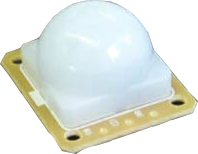
\includegraphics[width = .4\linewidth]{pir_sensor}
%	\caption{Passive infrared motion detector}
%\end{center}
%\end{figure}

%\begin{figure}[h]
%	\begin{center}
%		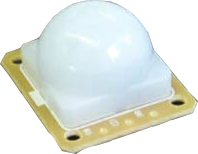
\includegraphics[width = .4\linewidth]{pir_sensor.png}
%		\caption{Passive infrared motion detector}
%	\label{fig:pirsensor}
%	\end{center}
%\end{figure}

%\begin{figure*}[t!]
%\centering
%\begin{subfigure}{.45\textwidth}
%  \centering
%  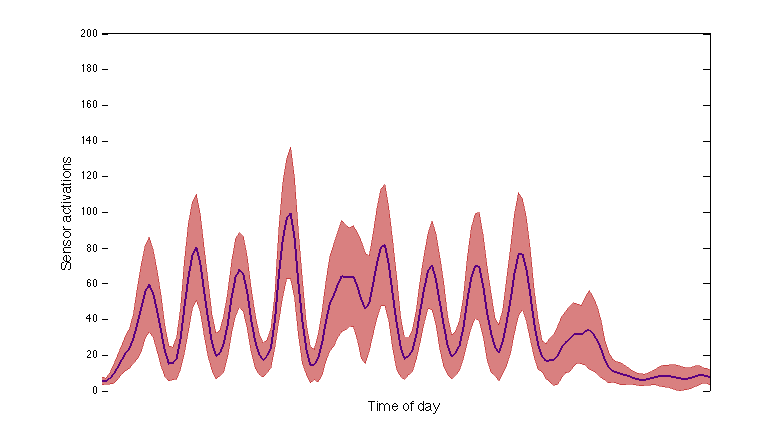
\includegraphics[width=1.0\linewidth]{brown_day.png}
%  \caption{CSM Brown Building average of all Wednesdays}
%  \label{fig:csmday}
%\end{subfigure}
%\begin{subfigure}{.45\textwidth}
%  \centering
%  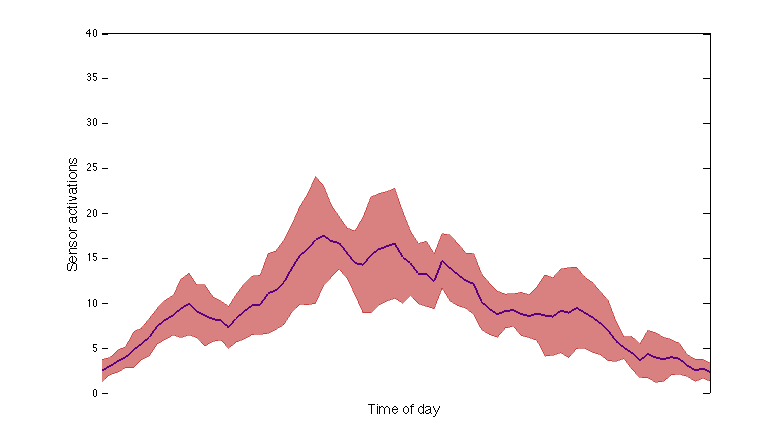
\includegraphics[width=1.0\linewidth]{merl_day.png}
%  \caption{MERL average of all Wednesdays}
%  \label{fig:merlday}
%\end{subfigure}
%\caption{Average sensor activations for a specific sensor on Wednesdays with one standard deviation range.}
%\label{fig:dayplot}
%\end{figure*}

This dataset is much different than the MERL dataset as classes typically provide activity on a rigid schedule during the day.  Also as students have exams and projects, late night motion is sporadic based on the time of year.  The counts of sensor activations have been aggregated over every 10 minutes.  Despite occasional late night motion during exam time, most nights have no significant motion.  For this reason we focus on data between 7:00am and 7:00pm daily.  A plot of the average activations of all Wednesdays for a single sensor along with a range of one standard deviation is given in Figure~\ref{fig:csmday}.  The defined peaks in the dataset correlate to class start and end times when most students will be in the hallways of the building.

\subsection{Denver traffic dataset}
Discuss the denver traffic dataset here.

\chapter{Models}
Discuss the relevant models which make up the BCF here.

\subsection{Seasonal ARIMA model}
The Auto Regressive Moving Average Model (ARMA) or derivations on its form (Auto Regressive Integrated Moving Average, Seasonal Auto Regressive Moving Average, $etc$) have been used in numerous forecasting applications from economics to vehicle traffic systems.  While we have been unable to find ARMA based models used on building occupancy data directly, we have found it used to forecast building energy usage and vehicle occupancy \cite{Williams2003, Hong2011, Newsham2010}.  Its forecasting accuracy is quite strong and it can serve as a strong baseline of comparison for a forecasting problem.  

Due to that fact that our building data has periodic trends and a non stationary mean, a seasonal ARIMA model is best suited to fit our data from the class of ARMA models.  The seasonal ARIMA model is defined as:
\begin{equation}
\label{eq:sarima}
\phi_{p}(B)\Phi_{p}(B^{s})\nabla^{d}\nabla^{D}_{s}T_{t} = \theta_{q}(B)\Theta_{Q}(B^{s})e_{t}
\end{equation}
\noindent
where $\{T_{t}\}$ is our observed time series and $\{e_t\}$ represents an unobserved white noise series ($e_{t} \sim N(0, \sigma^{2})$ )the values of which are computed through model training and are not known a priori.  $B$ is the backshift operator which is a function that allows access to older time readings.  For example $BT_{t} = T_{t-1}$ and $B^{5}T_{t} = T_{t-5}$.  $\nabla^{D}_{s}$ is the seasonal difference operator ($\nabla^{D}_{s}T_{t} = (1 - B^{s})^{D}T_{t}$)and $\phi,\  \Phi,\  \theta,\ \Theta$ are trainable parameters.  

Seasonal ARIMA models are notated as
\begin{equation}
ARIMA(p,d,q)(P,D,Q)_{s}
\end{equation}
where $p$ is the number of autoregressive terms, $d$ is the number of differences and $q$ is the number of moving average terms.  $P$, $D$, and $Q$ all correspond to the seasonal equivalents of $p$, $d$, and $q$.  The parameter $s$ is the seasonality of the model.  For a full discussion of seasonal ARIMA models see Box and Jenkins \cite{Box2008}.

Finding the correct values of $p, d, q, P, D, Q, s$ is traditionally a hard problem.  To fit our parameters we use a method similar to Williams \cite{Williams2003}.  As a verification of our model, we applied the LJung-Box test \cite{Ljung1978} on our set of residual data for each model.  This tests if any of the auto correlation values on the residual dataset are significantly different from 0.  To be valid, the LJung-Box test should return a value of $p > 0.05$.  Both residual sets passed: $p = 0.9964$ for MERL and $p = 0.1072$ for CSMBB.  Our final model parameters can be seen in Table~\ref{fig:sarimatab}.  Notice that the season is different for each model due to a difference in window of time for each day that we extracted data.

\begin{table}[t]
\centering
\caption{The parameter values that were fit for MERL and CSMBB datasets for a Seasonal ARIMA model}
\begin{tabular}{|c|c|c|c|c|c|c|c|} \hline
Dataset & $p$ & $d$ & $q$ & $P$ & $D$ & $Q$ & $s$\\ \hline
MERL & 0 & 0 & 1 & 0 & 1 & 5 & 78\\ \hline
CSMBB & 0 & 1 & 1 & 0 & 1 & 3 & 72\\ \hline
\end{tabular}
\label{fig:sarimatab}
\end{table}

Forecasting from this model is performed by iteratively forward feeding values of the model into itself.  Since the set of residuals $e$ from a properly trained seasonal ARIMA model is described by a white noise Gaussian distribution $N(0, \sigma^{2})$, we can take the expected value of the residual at time $e_{t + 1}$ to be 0.  This leaves us with the following forecasting equation: 
\begin{equation}
\label{eq:sarima}
\phi_{p}(B)\Phi_{p}(B^{s})\nabla^{d}\nabla^{D}_{s}T_{t + 1} = \theta_{q - 1}(B)\Theta_{Q - 1}(B^{s})e_{t}
\end{equation}

\subsubsection{Fitting a Seasonal ARIMA}
The underlying math of ARMA models stems from a linear filter operating on input from a stationary stochastic process.  ARIMA models were created to handle non-stationary data by differencing the data to induce stationarity.  Thus, a necessary step in fitting a ARIMA model to the data is first to determine the steps necessary to make the time series weakly stationary.  For a time series to be weakly stationary two conditions must be satisfied: The expected value of $x^{(t)}$ is the same for all $t$ and the covariance between any two observations depends only on the lag.  

In general it is difficult to prove stationarity, but there exists a number of methods which assist in determining if a time series is close enough to stationary to be modeled by an ARMA model.  Visual inspection of both the raw data and the autocorrelation function is a useful tool to test for stationarity.  Figure~\ref{fig:raw_data} shows the raw counts and autocorrelation values at hourly lags of vehicle counts for one sensor over a two week period.  The data shows no constant mean and thus can not be stationary.  The graph of autocorrelation values shows local peaks every 24 hours with a significant peak at one week of lag (168 hours).

Intuitively a one week seasonal difference should yield a stationary time series and visually, outside of an anomalous reading, Figure~\ref{fig:acf_lag} shows such stationarity.  Applying the Kwiatkowski-Phillips-Schmidt-Shin (KPSS) \cite{Kwiatkowski1992} test for stationarity on the seasonally differenced data confirms the visual inspection.  Using R's implementation of KPSS gives a p-value greater than 0.1.  This is significantly higher than the standard value to reject the stationarity hypothesis of 0.05.  

\begin{figure}[t]
\begin{center}
\subfloat[][Seasonal difference counts] {
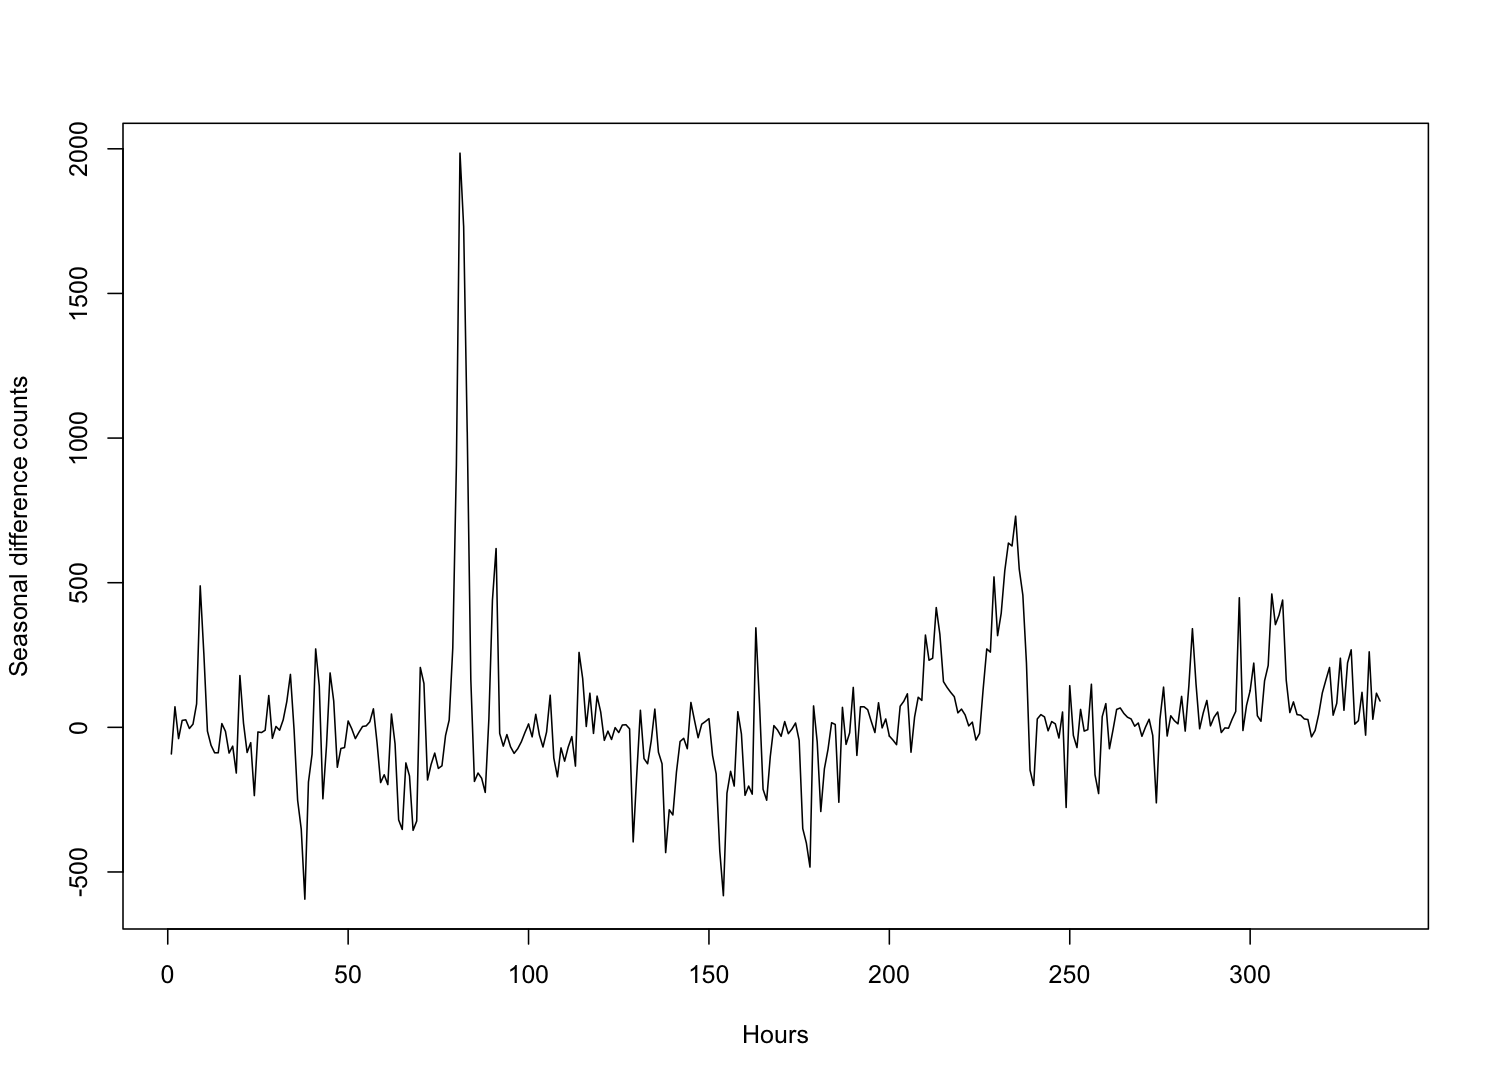
\includegraphics[width=0.45\textwidth]{lag_counts.png}
\label{fig:acf_counts}
}
\subfloat[][Autocorrelation of seasonal difference counts] {
\includegraphics[width=0.45\textwidth]{acf_lag.png}
\label{fig:acf_lag}
}
\end{center}
\caption{One week seasonal difference counts and autocorrelation over a two week period.}
\label{fig:lag_data}
\end{figure}

~\ref{fig:acf_counts}
~\ref{fig:lag_data}

Most of the input parameter values for seasonal ARIMA models tend to be 0, 1, 2, or 3 \cite{Box2008}.  Due to this small range of input values the total input space is relatively small (Six parameters with four possible values equates to $4^6 = 4096$) allowing us to apply a brute-force search for the best model.  Model performance is determined by the Akaike information criterion (AIC) \cite{Akaike1974}.  Our optimal model is a seasonal ARIMA $(1,0,1)(0,1,1)_{168}$.  

\begin{figure}[h]
\begin{center}
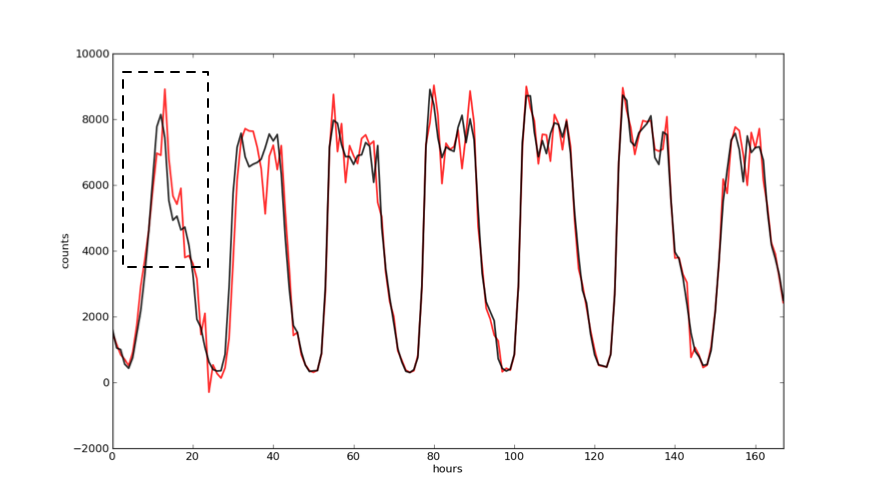
\includegraphics[width=0.8\textwidth]{broncos_predicted.png}
\end{center}
\caption{One-step ahead prediction for a sample week.  Black line is original data.  Red line is forecasted data.  Dotted box shows an example of mis-forecasting due to a broncos game.}
\label{fig:arima_prediction}
\end{figure}

Figure~\ref{fig:arima_prediction} shows an example of one-step ahead prediction performed on a sample week of test data.  The dotted line boxes a time when a Broncos game was occurring.  Forecasting during the Broncos game was initially low while traffic was unusually high as people were traveling to the game and then too high for much of the duration of the game.  This pattern of mis-forecasting is inline with the pattern demonstrated in Figure~\ref{fig:broncos_residual}.  The mean absolute percentage error (MAPE) for this week was approximately 8.2\%.  This MAPE is close to the results from other authors on other vehicle traffic datasets \cite{Williams2003,Smith1997}.  



\subsection{Historic average}
This model is simply the per day average of readings at each time step.  For certain types of data this model is has been shown to be more accurate than seasonal ARIMA forecasting \cite{Newsham2010}, specifically when the data has a strong historic correlation.  Average forecasts have the advantage of being extremely computationally fast and having a forecast accuracy that does not depend on the forecasting horizon.  This result will be shown later.

\subsection{Time delayed neural networks}

Time delayed neural networks are a special subset of regression neural networks where the input data is a local history of data from the time series.  Commonly the output is a single point forecast from that same time series at some point $t + \delta$ in the future.   The form of our 1 hidden layer time delayed neural network is:
\begin{equation}
T_{t + 1} = \phi \{ \sum_{j = 1}^{J} w_{j}\psi_{j} \bigg[ \sum_{l = 0}^{m}w_{ji}T_{t - l\delta} + w_{j0} \bigg] + w_0 \}
\end{equation}
\noindent where $\phi()$ is a linear activation function on the output layer and $\psi()$ is the standard sigmoid function.  A visual representation of the node architecture of a time delayed neural network is displayed in Figure~\ref{fig:tdnnarch}.

\begin{figure}[h]
	\centering
		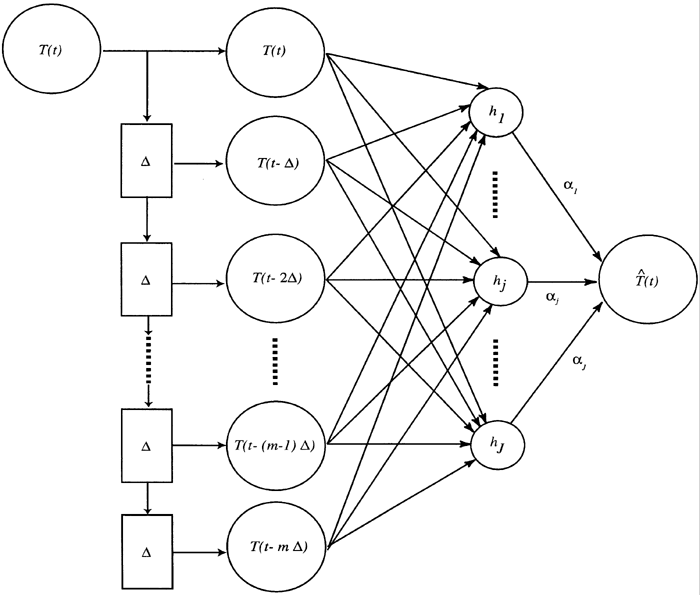
\includegraphics[width = .8\linewidth]{time_delay_neural_network.png}
		\caption{Architecture of a time delayed neural network with $m + 1$ inputs and J outputs \cite{Hansen2003}.}
	\label{fig:tdnnarch}
\end{figure}

Forecasting is performed by computing the output for a $m + 1$ length window of time and then iteratively forecasting a set of time steps in the future by using forecast data as inputs into the next forecast. 

The number of input nodes and hidden nodes for each dataset is given in Table~\ref{fig:tdnntab}.

\begin{table}[h]
\centering
\caption{Number of delayed input nodes and hidden nodes for MERL and CSMBB datasets}
\begin{tabular}{|c|c|c|} \hline
Dataset & Delayed input nodes & Hidden nodes\\ \hline
MERL & 15 & 8\\ \hline
CSMBB & 12 & 8\\ \hline
\end{tabular}
\label{fig:tdnntab}
\end{table}


\begin{table}[t!]
\centering
\caption{RMSE forecast values per model for a horizon equal to one.}
\begin{tabular}{|c|c|c|c|c|c|c|} \hline
Dataset & ARIMA & TDNN & AVG & SVM & BCF & BCF-TS\\ \hline
MERL & 5.5 & 2.67 & 4.35 & 2.29 & 2.28 & \textbf{2.26}\\ \hline
CSMBB & 10.94 & 14.13 & 27.14 & 11.01 & 8.72 & \textbf{8.72}\\ \hline
\end{tabular}
\label{fig:rmsetab}
\end{table}

\subsection{Support Vector Regression}
Support Vector Machine Regression (SVM) offers a powerful way to forecast time series.  It has been used in the past successfully to forecast travel times for vehicle traffic \cite{Wu2004}.  

As training SVM's is not done in the same way as other time series models, we first had to transform our dataset to a series of examples with a fixed window.  For a fixed window of size $w$, training input data is of the form $\{T_{t}, T_{t - 1}, ..., T_{t - w + 1}\}$.  Target data is of the form $T_{t + 1}$.  Thus the training examples which we provided to our SVM was $\{T_{t + 1}, [T_{t}, T_{t - 1}, ..., T_{t - w + 1}]\}$.

To perform SVM training we used the popular $libsvm$ package and as parameter selection is a notoriously difficult problem for SVM.  We followed the guidelines as outlined by Hsu, Chih-Chang and Lin, creators of the libsvm package \cite{Hsu2003}.  We first scaled the data by normalizing it between $[0, 1]$.  Then we searched for our best values of $C$, $\epsilon$ and $\gamma$ using the root mean squared error of the validation set a factor to determine performance of those parameters. 

For both the MERL and CSMBB datasets we used a window of 5.  This happened to be the same window length used by \cite{Wu2004}.

~\ref{fig:rmsetab}


\chapter{ENSEMBLE APPROACH}
write about approach here

\subsection{Bayesian Combined Forecasting}
The BCF approach \cite{Petridis2001} is one of several types of methods which attempt to combine other forecasting models for time series. We selected this forecasting method over other multiple model forecasting methods (such as mixture of experts or ensembles of neural networks) due to its modularity and strong statistical backing.  BCF is modular in that it allows for the component forecasting models to come from any trained forecaster with a well defined distribution of the forecaster's mis-forecasts.  Its statistical backing comes from its direct derivation from Bayes' rule.

This section derives the BCF approach for readers unfamiliar with it and then describes some modifications of the approach which improves its performance for our application.

\subsection{Notation}
We define the time series dataset used in these models as $\{T_{t}^{(m)}\}$.  In our application the data used for these models comes from a set of $M$ binary infrared sensors.  Each $T_{t}^{m}$ is a 10 minute aggregate of the readings from sensor $m$ reading at time block $t$.  

Forecasts for a given model $k$ from the set of all models $K$ are represented by 
\begin{equation}
\bar{T}_{t + 1}^{k, m} = f(T_{t}, ..., T_{1}; \theta_{k}).
\end{equation}
\noindent
Thus the forecast of $T_{t + 1}$ is a function of all past data and some trained parameterization $\theta_{k}$ for that model. 

In this work we need to forecast more than one time step into the future.  Future forecasts are performed through iterative one step ahead forecasts.  Also for this work we forecast a model for each individual sensor and for convenience drop the $m$ from our forecasting notation.  An example of a forecast two time steps ahead of current time $t$ is given by 
\begin{equation}
\bar{T}_{t + 2}^{k} = f(\bar{T}_{t + 1}, T_{t}, ..., T_{1}; \theta_{k}).
\end{equation}
\noindent
Such a forecast is simply the forecast for one time step into the future but now with the forecasted value of $\bar{T}_{t + 1}$ used as the most recent datapoint to forecast $\bar{T}_{t + 2}$.  Forecasting in this nature allows for forecasts any number of time steps into the future. 

\begin{figure*}[t]
\centering
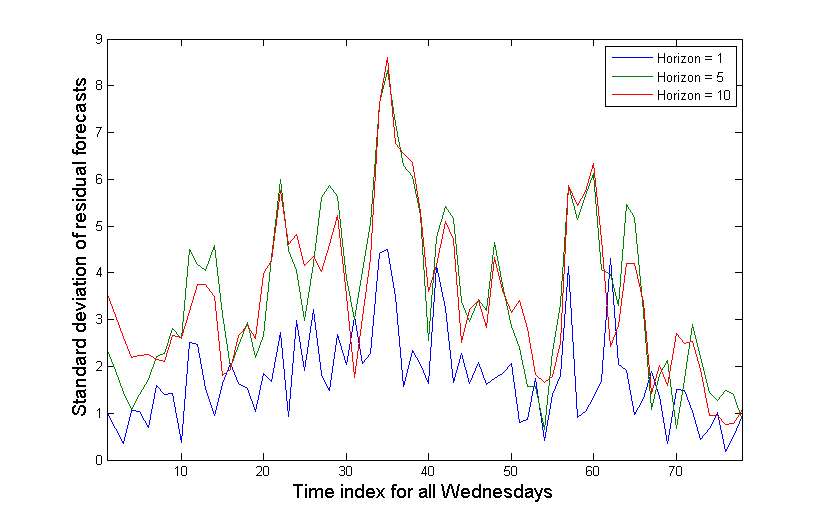
\includegraphics[width = .55\linewidth]{svm_standard_deviations_vs_horizon.png}
\caption{Standard deviation of support vector machine residuals for all Wednesdays in MERL dataset.  Time index represents 10 minute intervals from 6:00am to 7:00pm.}
\label{fig:svmstd}
\end{figure*}

\subsection{Bayesian Combined Forecasting Derivation}
To derive BCF we first assume the existence of $K$ models.  From these $K$ models, we want to create a probability distribution on a new random variable $z$ that is used to determine if model $k$ is the correct model from which to forecast at time $t$.  To do this we use the notation of Petridis \cite{Petridis2001} and define $p_{t}^{k}$ as follows
\begin{equation}
p_{t}^{k} = p(z = k | T_{t}, ..., T_{1}).
\end{equation}

From here we apply Bayes rule and get
\begin{equation}
p_{t}^{k} = \frac{p(T_{t} | z = k, T_{t - 1}, ..., T_{1}) \cdot p(z = k | T_{t - 1}, ..., T_{1})} {p(T_{t}, ..., T_{1})}.
\end{equation}
\noindent
Notice that $p(z = k | T_{t - 1}, ..., T_{1}) = p_{t - 1}^{k}$.  Thus we can create a recursive estimation based on prior $p_{t}^{k}$.

With recursive values for $p_{t}^{k}$ and replacing $p(T_{t}, ..., T_{1})$ with a conditional probability on $z$ we get
\begin{equation}
p_{t}^{k} = \frac{p(T_{t} | z = k, T_{t - 1}, ..., T_{1}) \cdot p_{t - 1}^{k}} {\sum_{j = 1}^{K}p(T_{t} | z = j, T_{t - 1}, ..., T_{1}) \cdot p_{t - 1}^{j}}.
\end{equation}

We use the empirically observed forecasting error for each model to estimate $p(T_{t}|z = k, T_{t - 1}, ..., T_{1})$.  The forecasting error for a given model at time $t$ is 
\begin{equation}
e_{t}^{k} = \bar{T}_{t}^{k} - T_{t}.
\end{equation}
\noindent
We can use these forecasting errors to estimate a probability distribution for each model on the random variable $e_{t}^{k}$.  This is typically modeled as a white noise zero mean Gaussian process.  For our work, we represent this as a distribution of error terms with some parameterization $\omega_{k}$.  Thus for each model the probability error distribution function on the model error random variable is given by $q(e_{t}^{k};\omega_{k})$.

The final equation for the posterior probability of a given model $k$ is
\begin{equation}
\label{eq:model_prob}
p_{t}^{k} = p(z = k|T_{t}, ..., T_{1}) = \frac{p_{t - 1}^{K} \cdot q(T_{t} - \bar{T}_{t}^{k}; \omega_{k})}{\sum_{j=1}^{K}p_{t - 1}^{j} \cdot q(T_{t}^{j} - \bar{T}_{t}^{j}; \omega_{j})}.
\end{equation}

An example of these changing normalized posterior probabilities for a small section of the MERL dataset is shown in Figure~\ref{fig:probsmerl}.

Forecasting using BCF is done by either computing a weighted forecast $\delta$ time steps into the future for each forecasting model or by simply selecting the model with the highest likelihood.  For this paper we forecast using a weighted forecast of all models.  The forecasting equation is
\begin{equation}
T_{t + \delta}^{ALL} = \sum_{k=1}^{K}p_{t}^{k} \cdot \bar{T}_{t + \delta}^{k}.
\end{equation}

\begin{figure}
\centering
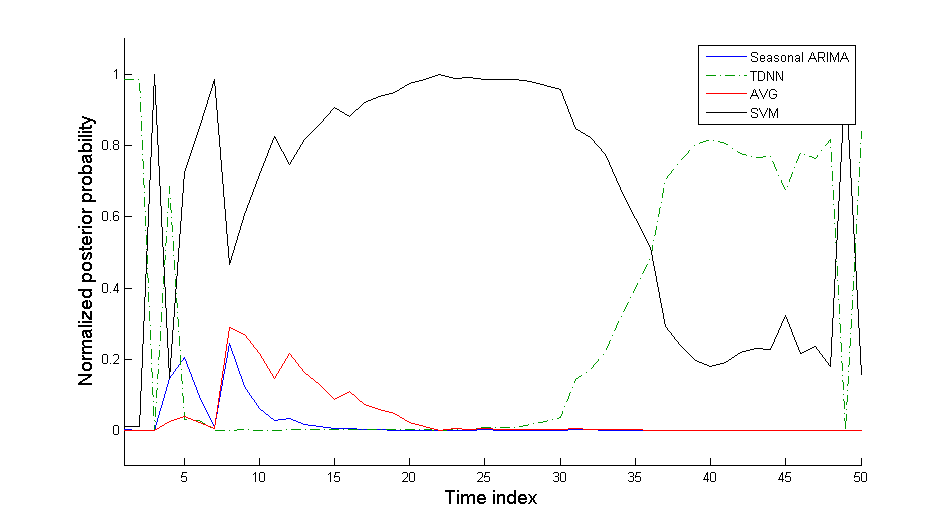
\includegraphics[width = 1.0\linewidth]{posterior_probs.png}
\caption{Normalized posterior probabilities of component models on a section of MERL dataset.}
\label{fig:probsmerl}
\end{figure}

\subsection{BCF Modifications}
In this subsection we discuss a number of modifications to maximize the effectiveness of BCF for our data.  We refer to the modified BCF algorithm as Bayesian Combined Forecasting for multiple Time Steps or BCF-TS for short.  These modifications  enable BCF to work with forecasting horizons greater than one in the future.

\subsubsection{Forecast $\delta$ time steps into the future}
Traditional implementations of BCF in other domains \cite{Petridis2001, Zheng2006} are interested only in 1 time step ahead forecasts.  For our work we require forecasts that are $\delta$ steps ahead which requires a small change to the BCF method.  Instead of generating a model's error distribution from 
\begin{equation}
e^{t}_{k} = \bar{T}_{t}^{k} - T_{t} = f(\bar{T}_{t},T_{t - 1} ..., T_{1}; \theta_{k}) - T_{t}.
\end{equation}

The error distribution is instead generated from 
\begin{equation}
e^{t}_{k} = f(\bar{T}_{t}, ..., \bar{T}_{t - \delta + 1}, T_{t - \delta}, ..., T_{1};\theta_{k}) - T_{t}.
\end{equation}
The reason for this change is due to the assumption that our error distribution is an accurate representation forecasting accuracy.  
The forecasting error distribution for models at $1$ time step into the future is not necessarily the same as models at $\delta$ time steps.  Thus we compute a different error distribution for each forecast time step.


\subsubsection{Improving model error distributions}
Despite other implementations of BCF using fixed error distributions, our data has clear daily trends.  For some of our models, the forecasted residuals follow these same trends.  See Figure~\ref{fig:svmstd} for an example of how the forecasting error distribution for a trained support vector regression model on the MERL dataset depends on the time and on the forecasting horizon.

To represent a more realistic error distribution instead of a fixed white noise Gaussian that is commonly used in the literature, we fit a Gaussian for each 10 minute slice of a given day.  The data from the MERL dataset was used from 6:00am to 7:00pm. The thirteen hours of data used per day represent 78 time slices.  For example taking the data for each time slice for each Wednesday results in 78 Gaussian error distributions for each forecasting horizon.  These Gaussians are computed from a validation set representing 20\% of our data.  It is from this set of models error distributions that we compute BCF.

As a possible improvement to this set of error distributions, we note that using a generalized autoregressive conditional heteroskedastic (GARCH) model \cite{Box2008} or some other appropriate model to forecast future variance based on local and historic changes in variance would likely outperform our time based average Gaussian models.  GARCH models are similar to seasonal autoregressive moving average models which we use as one of our component forecasting models.

\subsubsection{Model selection thresholding}
Diebold \cite{Diebold1991} cautions against the use of forecasting using a Bayesian combination of models in all cases.  Diebold points out that under certain situations a convex combination of forecasts for models may not be optimal, and cases exist where taking negative likelihood weighting may be optimal.  These conditions are likely to arise during instances where the data may not be accurately described by any of the forecasting models.  

Furthermore when such cases where no model is able to provide an accurate forecast, then it is often the case that forecasts come from the worst model.  

To combat this case, we have implemented a model selection threshold $h_{k}$.  If the likelihood of all component models is below $h_{k}$, then we forecast from only the model which is historically the most accurate based on our validation set.  

The threshold is different for each model, and should depend on the error distribution of the model.  In practice we have found that $2\sigma$ serves as a good threshold.  Basing the threshold on $\sigma$ is useful as it provides a threshold value which does not depend on $e^{k}_{t}$.  For a zero mean Gaussian the probability of the $2\sigma$ threshold is
\begin{equation}
p(2\sigma) = \frac{1}{\sigma\sqrt{2\pi}}e^{-2}.
\end{equation}
Because the Bayesian combined forecasting approach is iterative, it is possible that a long section of forecasts that indicate one model correct or incorrect can lead to likelihood underflow.  Due to this problem we adjust our normalized likelihoods so that no model may reach a value below 0.001.  This empirically chosen value is low enough to not have a great impact on forecasts while still being high enough to allow model likelihoods to change quickly.

\subsection{Results of Ensemble}

BCF and BCF-TS (BCF with our specific set of modifications) were trained and tested using all component models described above.  All of the models were trained on 60\% of the total datasets.  Another 20\% was used for model validation and the final 20\% used for testing.  All results shown below are on the test set only.  Figure~\ref{fig:realbcf} shows an sample section of test data from the MERL dataset along with BCF-TS forecasts for horizons of 1 and 5.   As expected as the forecasting horizon increases the forecasts become less accurate.

\begin{figure}[h]
\centering
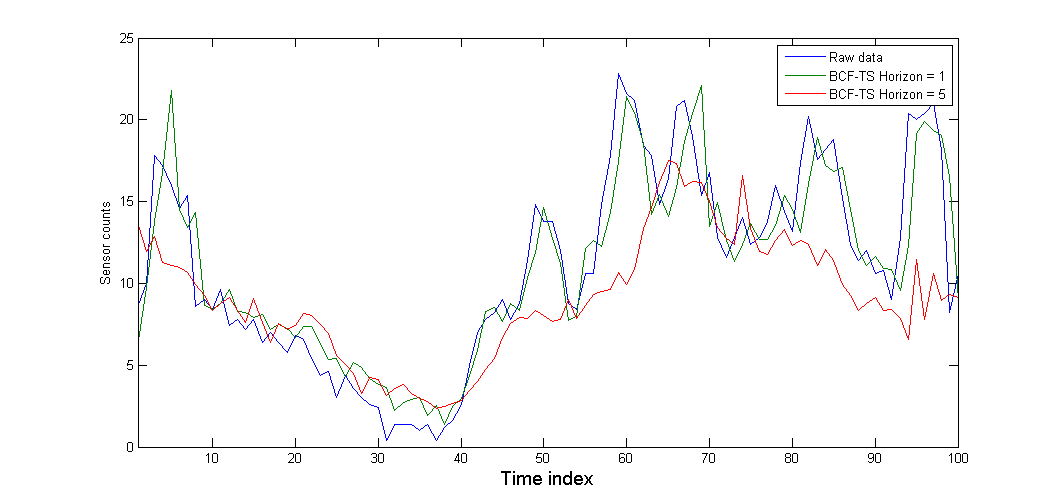
\includegraphics[width = 1.0\linewidth]{real_forecasts_bcf.png}
\caption{A comparison of forecasts at various horizons against real data for an sample time segment using BCF-TS.}
\label{fig:realbcf}
\end{figure}

It is common for one model's normalized posterior probability to be near one when that model is currently accurate.  Figure~\ref{fig:realbcfsvm} shows as example of this behavior.  From time index 1 to 8, the SVM component model has a posterior probability near 1.0 and as a result BCF-TS forecasts nearly completely from this model.  Then from time index 9 on the model's posterior probability is lower and as a result BCF-TS uses other model for its combined forecast.

\begin{figure}[h]
\centering
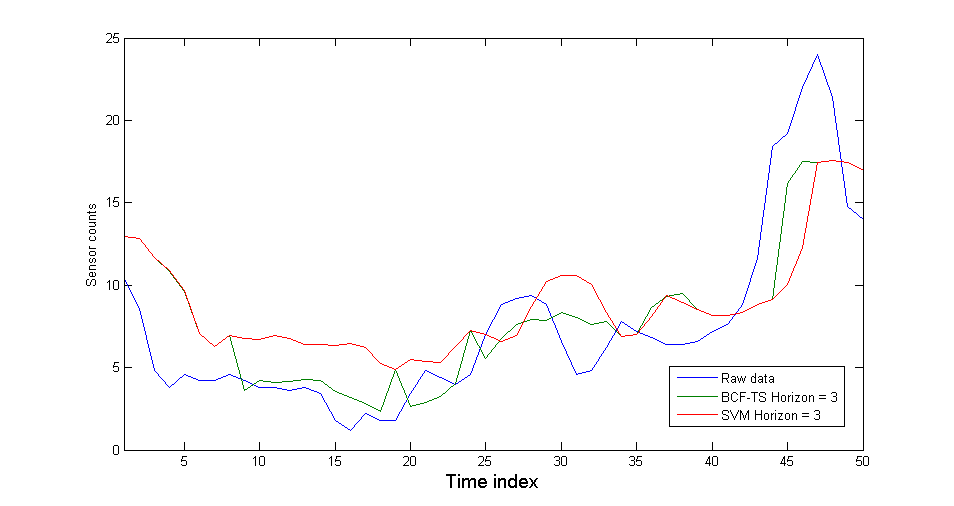
\includegraphics[width = 1.0\linewidth]{real_forecasts_bcf_svm.png}
\caption{A comparison of BCF-TS and SVM forecasts at horizon equal to three against real data.}
\label{fig:realbcfsvm}
\end{figure}

Figure~\ref{fig:rmseplot} shows the results of the root mean squared error (RMSE) of forecasts across a forecast horizon up to 10 time steps (100 minutes) into the future for each model.  These plots show that BCF-TS has the lowest error.  However, the average model shows itself to be a strong indicator of future activity for forecasts beyond 60 minutes into the future.  Forecasts were performed for significantly longer horizons, but the results were uninteresting as the total RMSE of models converged to roughly the values at a forecasting horizon of 10 time steps.  

\begin{table}
\centering
\caption{Run times (in seconds) for each forecasting horizon.}
\begin{tabular}{|c|c|c|c|c|c|c|c|} \hline
Algorithm & $1$ & $2$ & $3$ & $5$ & $8$ & $10$ \\ \hline
Average & 0.001 & 0.001 & 0.001 & 0.001 & 0.001 & 0.001 \\ \hline
ARIMA & 0.043 & 0.045 & 0.046 & 0.053 & 0.058 & 0.063\\ \hline
SVM & 0.048 & 0.910 & 0.137 & 0.227 & 0.357 & 0.444 \\ \hline
TDNN & 20.87 & 21.60 & 21.82 & 21.28 & 22.73 & 22.50 \\ \hline
BCF-TS & 20.97 & 21.26 & 21.27 & 21.34 & 21.57 & 21.63\\ \hline
\end{tabular}
\label{fig:runtimestab}
\end{table}

In the CSMBB dataset the Seasonal ARIMA model was a good forecaster of future activity while in the MERL set it performed significantly worse than even the average model on all forecasting horizons.  This is likely due to a stronger seasonal component to the CSMBB dataset due class schedules.  Instead on the MERL dataset there is little seasonal correlation and thus natural variance from a prior season may incorrectly affect current forecasts.  This result is similar to that of other papers that use seasonal ARIMA models \cite{Newsham2010}; where in the case of strong seasonal data, results are better for short horizon forecasts, but longer forecasts favor historic averages.

BCF and BCF-TS were both better at a horizon of one time step for all component models (see Table~\ref{fig:rmsetab}).  In the MERL dataset standard BCF was outperformed by SVM and later the average model for all forecast beyond one horizon.  However the BCF-TS model showed significant improvement in RMSE scores for all forecasting horizons unto 60 minutes.  For horizons of 10 time steps and greater, the average model is about as good as the BCF-TS approach.

Table~\ref{fig:runtimestab} shows the run time in seconds of each forecasting algorithm at a given forecasting horizon.  The times are for forecasting the entire test set on the MERL dataset for a single sensor, approximately twenty weeks worth of data.  In general BCF-TS was slower than any component model, but the times are still such that real-time forecasting is possible.

\begin{figure}[!ht]
	\begin{center}
		\subfigure[] {
			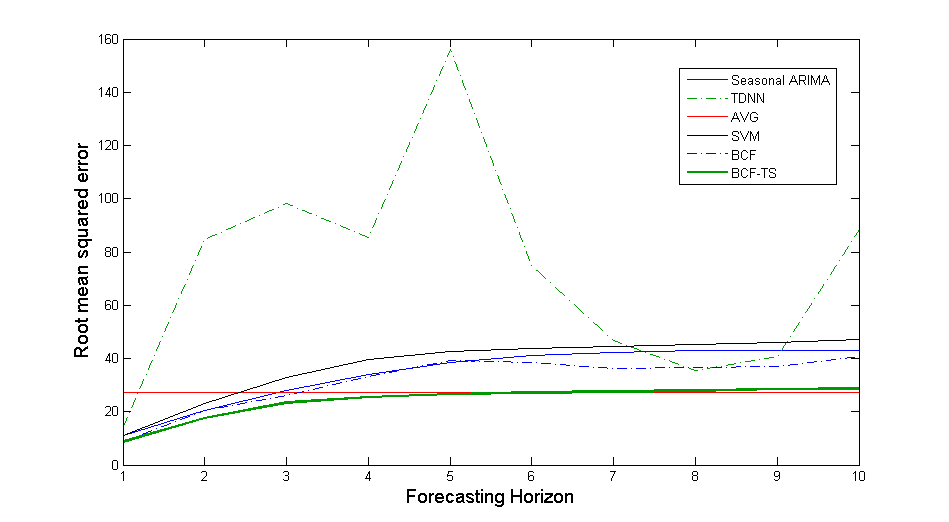
\includegraphics[width=0.49\linewidth]{brown_rmse.png}
			%\caption{CSMBB forecasting model errors}
			%\label{fig:csmrmse}
		}
		\subfigure[] {
			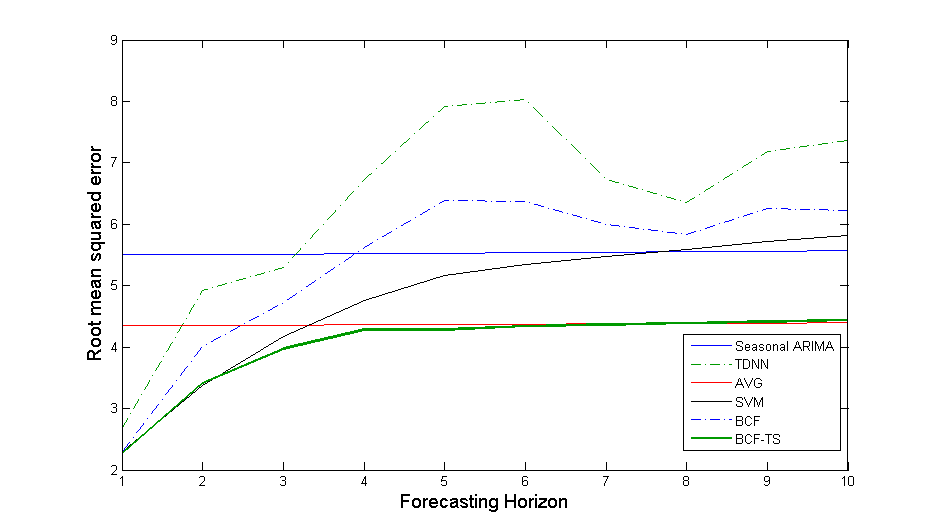
\includegraphics[width=0.49\linewidth]{merl_rmse.png}
			%\caption{MERL forecasting model errors}
			%\label{fig:merlrmse}
		}
	\end{center}
	\caption{Root mean square error of forecasting for each model vs forecasting horizon.}
	\label{fig:rmseplot}
\end{figure}




\chapter{Improved Ensemble}
Discuss our improved ensemble method here

\subsection{Activity recog}
discuss activity recognition and its importance here

\subsection{HMM vs TSMG}
discuss why we are not using hidden markov models as stated in the proposal

\subsection{TSMG derivation}

A mixture of Gaussians is a strongly supported stochastic data clustering technique used in activity recognition.  Traditionally, a mixture of Gaussians is implemented for either a one dimensional time series (CITE PAPER TO SUPPORT THIS) or for data vectors with no time element.  Here we combine the two approaches, creating a mixture of Gaussians for multi-dimensional time series data.  While this approach has not yet been implemented, based on the success of mixture of Gaussians in other domains, we expect good results.

The goal of mixture of Gaussians is to find a set of models which will maximize the log likelihood of the parameters of some models to the dataset.  Given dataset $\{x^{(i)}\}$ we maximize
\begin{equation}
\ell(\theta) = \sum_{i = 1}^{\bf M}log\{p(x^{(i)}|\theta)\}
\end{equation}
\noindent 
where ${\bf M}$ is the total number of time series instances.

The expectation maximization (EM) algorithm is commonly used to maximize dataset likelihood.  To use this algorithm we need to define a set of variables
\begin{equation}
w_{k}^{(i)} = p(z = k|x^{(i)})
\end{equation}
\noindent
where ${\bf K}$ is the total number of Gaussians to train and $k$ is an index of ${\bf K}$.  

The general equation for the likelihood of the models is: 
\begin{equation}
\label{eq:em_likelihood}
\ell(\theta|x) = \sum_{i = 1}^{{\bf M}}\sum_{k = 1}^{{\bf K}}w_{k}^{(i)}\log \{ \frac{p(x^{(i)}|z=k)p(z = k)}{w_{k}^{(i)}} \}
\end{equation}

In the traditional mixture of Gaussians algorithm each model is ostensibly a Gaussian.  To make this algorithm work with multi-dimensional time series, we define the models instead by
\begin{equation}
\label{eq:model}
p(x^{(i)}|z = k) = \prod_{n = 1}^{{\bf N}}\mathcal{N}_{n}(x^{(i)})
\end{equation}
\noindent
where ${\bf N}$ is the length of each time series instance.  Thus our model for each time series is ${\bf N}$ independent multivariate Gaussians.

Combining equations~\ref{eq:em_likelihood} and~\ref{eq:model} gives the following log likelihood
\begin{equation}
\label{eq:em_combined}
\ell(\theta|x) = \sum_{i = 1}^{{\bf M}}\sum_{k = 1}^{{\bf K}}w_{k}^{(i)}\{ \log\frac{p(z = k)}{w_{k}} + \sum_{n = 1}^{{\bf N}} \log \mathcal{N}_{n}(x^{(i)})\}
\end{equation}

\textbf{E-Step}
The E-step hardly changes from the traditional EM mixture of Gaussians algorithm.  We simply need to calculate 
\begin{equation}
w^{(i)}_{k} = p(z = k|x^{(i)})
\end{equation}

\textbf{M-Step}
For the maximization step, it is assumed that we know the values of $w_{k}^{(i)}$.  Thus, we need to maximize equation~\ref{eq:em_combined} with respect to $\mu$,  $\Sigma$, and $\theta$.
The results of these maximizations are given below:
\begin{equation}
\theta_{k} = \frac{1}{{\bf M}}\sum_{i = 1}^{{\bf M}}w_{k}^{(i)}
\end{equation}
\begin{equation}
\mu_{k, n} = \frac{\sum_{i = 1}^{{\bf M}}w_{k}^{(i)}x^{(i)}_{n}}{\sum_{i = 1}^{{\bf M}}w_{k}^{(i)}}
\end{equation}
\begin{equation}
\Sigma_{k, n} = \frac{\sum_{i = 1}^{{\bf M}}w_{k}^{(i)}(x^{(i)} - \mu_{k, n})(x^{(i)} - \mu_{k, n})^{\mathrm{T}}}{\sum_{i = 1}^{{\bf M}}w_{k}^{(i)}}
\end{equation}


\subsection{Improved Ensemble Derivation}
Derive our improved ensemble method here.




\chapter{conclusion}
Discuss our conclusions here

%%% Below is a quick test for a figure that moves to another page
% asdfadsf
% 
% asdfasdf
% 
% dfsdfds
% 
% dsfsd
% 
% sdfdsfd
% %% Note: the ''[H]`` below is optional and means ''always put it exactly here``, normally you do NOT want to use it.  However, in some rare circumstances you may wish to override the default placement.
% \csmfigure[H]{Stomata}{figures/stomata}{4in}{A pretty picture from the Squier Group --- this is a test of the emergency long-title system.}
%%% End special test

%%%%%%%%%%%%%%%%%%%%%%%%%%%%%%%%%%%%%%%%%%%%%%%%%%%%%%%%%%%%%%%%%%%%%%%%%%%%%%%%%%%%%%%%%%%%%
% If you would like to work on each chapter of your thesis in a separate document then use: %
%%%%%%%%%%%%%%%%%%%%%%%%%%%%%%%%%%%%%%%%%%%%%%%%%%%%%%%%%%%%%%%%%%%%%%%%%%%%%%%%%%%%%%%%%%%%%
%% Parts of a Thesis - Back Matter
%\backmatter

%%% Parts of a Thesis - Back Matter - References Cited (required)

% Use "Advanced" Bibliography Techniques
\bibliography{Final_Thesis}
\end{document}
